\section{边界模式}
\label{sec:heat-modes}

三角形的形状一直在变，直接跟踪它并不方便。换一个问法：有没有这样的初始形状，演化时形状不变，只是整体按比例缩小？如果有足够多这样的形状，任何初值都可以拆开，各部分分别衰减，再加回去。

\paragraph{离散后的特征向量}
把棒离散成向量，问题就是我们熟悉的。取步长$h=1/4$，内部三个格点$x_j=j/4$，端点取零，用二阶差商代替$\partial_x^2u$，记$\bm{u}(t)$为三个格点上的温度。方程成为线性常微分方程组
\[
 \dot{\bm{u}}=-\bm{K}\bm{u},\qquad
 \bm{K}=16\begin{bmatrix}2&-1&0\\-1&2&-1\\0&-1&2\end{bmatrix} .
\]
矩阵的特征向量正是“形状不变”的初值：若$\bm{K}\bm{v}=\mu\bm{v}$，从$\bm{v}$出发的解是$\mathrm{e}^{-\mu t}\bm{v}$。

三个特征值和特征向量可以手算验证。取$\bm{v}=(\sqrt2/2,\,1,\,\sqrt2/2)^{\top}$，第一行给出$16(\sqrt2-1)\approx6.627$，第二行给出$16(2-\sqrt2)\approx9.373$，比值都是$9.373$，这就是$\mu_1$。全部结果是
\[
 \mu_1=16(2-\sqrt2)\approx9.37,\quad \mu_2=32,\quad \mu_3=16(2+\sqrt2)\approx54.63 .
\]
特征向量恰好是$\sin(k\pi x)$在格点上的取值，$k=1,2,3$，见图~\ref{fig:heat-discrete-modes}。这提示连续问题的“特征向量”是正弦函数，对应的$\mu_k$则应当逼近某个随$k$增长的数。

\begin{BookInlineFigure}
  \centering
  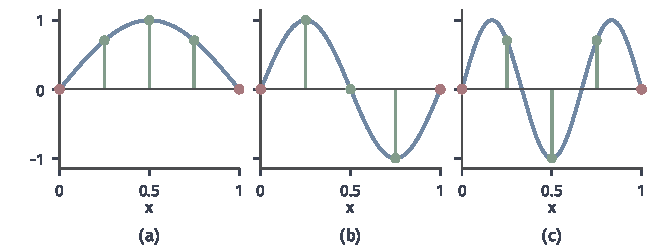
\includegraphics[width=112mm]{figures/06-differential-equations/02-partial-differential-equations/matplotlib/heat-discrete-modes/figure.pdf}
  \caption{三个内部格点的离散问题。绿色竖线是矩阵$\bm{K}$的三个特征向量，蓝线是$\sin(k\pi x)$，红点是固定为零的端点。(a)$k=1$。(b)$k=2$。(c)$k=3$。}
  \label{fig:heat-discrete-modes}
\end{BookInlineFigure}

\paragraph{分离变量}
现在回到连续问题，令$f=0$，寻找形如$u(x,t)=\varphi(x)a(t)$的解，这种做法称为\term{分离变量}（separation of variables）。代入$\partial_tu=\partial_x^2u$，得到
\[
 \varphi(x)\,a'(t)=\varphi''(x)\,a(t) .
\]
在$\varphi$和$a$不为零的地方两边相除，
\[
 \frac{a'(t)}{a(t)}=\frac{\varphi''(x)}{\varphi(x)} .
\]
左边只依赖$t$，右边只依赖$x$，二者相等只能都是常数，记作$-\lambda$。于是偏微分方程分成两个常微分方程：
\begin{equation}
 a'=-\lambda a,\qquad -\varphi''=\lambda\varphi .
 \label{eq:heat-separated}
\end{equation}

时间方程的解是$a(t)=a(0)\mathrm{e}^{-\lambda t}$。空间方程加上边界条件，只对某些$\lambda$有非零解，这称为\term{边界特征值问题}（boundary eigenvalue problem）。边界条件正是在这里进入：它决定哪些形状可用。

\paragraph{Dirichlet边界的模式}
要求$\varphi(0)=\varphi(1)=0$，按$\lambda$的符号分三种情形。

若$\lambda<0$，记$\omega=\sqrt{-\lambda}$，通解是$\varphi=A\cosh\omega x+B\sinh\omega x$。由$\varphi(0)=0$得$A=0$，由$\varphi(1)=B\sinh\omega=0$得$B=0$，没有非零解。

若$\lambda=0$，通解是$\varphi=A+Bx$，两个端点条件同样迫使$A=B=0$。

若$\lambda>0$，记$\omega=\sqrt\lambda$，通解是$\varphi=A\cos\omega x+B\sin\omega x$。由$\varphi(0)=0$得$A=0$。要有非零解，必须$\sin\omega=0$，即$\omega=k\pi$。把振幅归一化后，全部模式是
\begin{equation}
 e_k(x)=\sqrt2\sin(k\pi x),\qquad \lambda_k=k^2\pi^2,\qquad k=1,2,\ldots .
 \label{eq:heat-dirichlet-modes}
\end{equation}

与离散结果比较，连续问题的前三个特征值是
\[
 \lambda_1\approx9.87,\quad \lambda_2\approx39.5,\quad \lambda_3\approx88.8 .
\]
低频的$\mu_1$已经接近$\lambda_1$，高频差别较大，三个格点本来就表示不好高频。

每个模式独立地按$\mathrm{e}^{-k^2\pi^2t}$衰减，频率越高衰减越快。振幅减半的时间是$\ln2/\lambda_k$：$k=1$时约$0.0702$，$k=3$时约$0.0078$，相差九倍。原因就是前面的邻居平均：振荡越快，峰与邻居的落差相对越大。图~\ref{fig:heat-mode-decay}(a)的初值是$\sin(\pi x)+\tfrac12\sin(4\pi x)$，小起伏很快消失，大的拱形缓慢下降；图~\ref{fig:heat-mode-decay}(b)在对数坐标中把衰减画成直线，斜率是$-\lambda_k$。

\begin{BookInlineFigure}
  \centering
  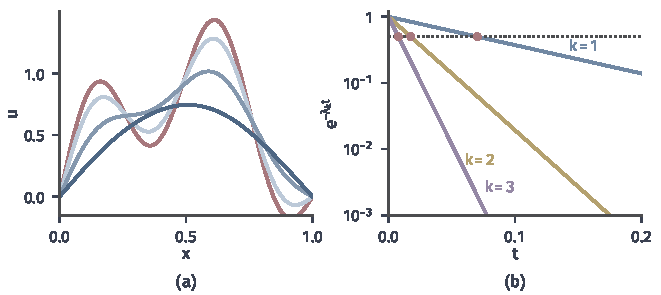
\includegraphics[width=112mm]{figures/06-differential-equations/02-partial-differential-equations/matplotlib/heat-mode-decay/figure.pdf}
  \caption{模式衰减。(a)初值$\sin(\pi x)+\tfrac12\sin(4\pi x)$（红）与$t=0.002,0.008,0.03$的解（蓝色由浅到深）。(b)$k=1,2,3$的振幅因子，纵轴为对数刻度，红点是振幅减半的时刻，虚线高度为$1/2$。}
  \label{fig:heat-mode-decay}
\end{BookInlineFigure}

\paragraph{Neumann边界的模式}
把边界换成$\varphi'(0)=\varphi'(1)=0$，计算只有一处结果不同。$\lambda<0$时，$\varphi'=\omega(A\sinh\omega x+B\cosh\omega x)$，由$\varphi'(0)=0$得$B=0$，由$\varphi'(1)=0$得$A=0$，仍无非零解。$\lambda>0$时，由$\varphi'(0)=0$得$B=0$，再由$\sin\omega=0$得$\omega=k\pi$。

不同的是$\lambda=0$：$\varphi=A+Bx$的导数是$B$，只要$B=0$就满足两个条件，常数活了下来。全部模式是
\begin{equation}
 \tilde{e}_0(x)=1,\quad\lambda_0=0;\qquad \tilde{e}_k(x)=\sqrt2\cos(k\pi x),\quad\lambda_k=k^2\pi^2\quad(k\geq1) .
 \label{eq:heat-neumann-modes}
\end{equation}

$\lambda_0=0$的模式称为\term{零模式}（zero mode），它的时间因子恒为$1$，永远保留。常数没有曲率，每一点都等于邻居的平均值，没有理由变化。这与表~\ref{tab:heat-boundary-compare}的总热量守恒相合：隔热棒里的热量无处可去，它最后全部留在这个常数里。

\paragraph{初值如何确定系数}
要用这些模式表示一般的初值，需要两件事：模式彼此正交，模式足够多。正交性可以直接算。对$j\neq k$，由积化和差，
\[
 \int_0^12\sin(j\pi x)\sin(k\pi x)\,\mathrm{d}x
 =\int_0^1\bigl(\cos((j-k)\pi x)-\cos((j+k)\pi x)\bigr)\,\mathrm{d}x=0 ,
\]
$j=k$时同样的式子给出$1$。

完备性来自Fourier级数：把$(0,1)$上的函数奇延拓到$(-1,1)$，再按周期$2$展开，余弦系数全为零，只剩$\sin(k\pi x)$；偶延拓则只剩余弦。所以$\{e_k\}_{k\geq1}$与$\{\tilde{e}_k\}_{k\geq0}$都是$L^2(0,1)$的标准正交基，三角系统的完备性可参考\BookChapterRef{chap:fourier-transform}{卷四第14章“Fourier变换”}。

于是对$u_0\in L^2(0,1)$，令$c_k=\langle u_0,e_k\rangle$，就有$u_0=\sum_kc_ke_k$（在$L^2$中收敛）和Parseval等式$\sum_kc_k^2=\lVert u_0\rVert_2^2$。把每一项换成衰减后的形式，就得到候选解。它是否真的是解，初值在什么意义下恢复，需要证明。

\begin{theorem}[区间上的模式解]
\label{thm:heat-series}
设$u_0\in L^2(0,1)$，$c_k=\langle u_0,e_k\rangle$，$\lambda_k=k^2\pi^2$，令
\begin{equation}
 u(x,t)=\sum_{k\geq1}c_k\mathrm{e}^{-\lambda_kt}e_k(x) .
 \label{eq:heat-sine-solution}
\end{equation}
则下列结论成立。
\begin{enumerate}
 \item 对每个$t\geq0$，级数在$L^2(0,1)$中收敛，满足
 \begin{equation}
  \lVert u(\cdot,t)\rVert_2\leq\mathrm{e}^{-\pi^2t}\lVert u_0\rVert_2,
  \label{eq:heat-series-decay}
 \end{equation}
 并且$t\to0^+$时$\lVert u(\cdot,t)-u_0\rVert_2\to0$。
 \item 级数及其任意阶逐项导数在$[0,1]\times[t_0,\infty)$上一致收敛（$t_0>0$），所以$u$在$[0,1]\times(0,\infty)$上无穷次可微，逐点满足热方程和零边值。
 \item 若$u_0$连续、分段连续可微且$u_0(0)=u_0(1)=0$，则$\sum_k\lvert c_k\rvert<\infty$，$u$在$[0,1]\times[0,\infty)$上连续，$u(\cdot,0)=u_0$处处成立，$u$是定义~\ref{def:heat-ibvp}意义下的经典解。
\end{enumerate}
\end{theorem}

\begin{proof}
(1)由Parseval等式，系数$c_k\mathrm{e}^{-\lambda_kt}$平方可和，级数收敛。又$\lambda_k\geq\pi^2$，所以
\[
 \lVert u(\cdot,t)\rVert_2^2=\sum_kc_k^2\mathrm{e}^{-2\lambda_kt}\leq\mathrm{e}^{-2\pi^2t}\sum_kc_k^2 .
\]
这就是式~\eqref{eq:heat-series-decay}。初值的恢复同样按坐标计算：
\[
 \lVert u(\cdot,t)-u_0\rVert_2^2=\sum_kc_k^2\bigl(1-\mathrm{e}^{-\lambda_kt}\bigr)^2 .
\]
每一项在$t\to0^+$时趋于零，且不超过可和的$c_k^2$，由级数的控制收敛定理，和趋于零。

(2)由Parseval等式，$\lvert c_k\rvert\leq\lVert u_0\rVert_2$。对$x$求$m$次、对$t$求$n$次后，第$k$项在$t\geq t_0$上的绝对值不超过
\[
 \sqrt2\,\lVert u_0\rVert_2\,(k\pi)^{m+2n}\,\mathrm{e}^{-k^2\pi^2t_0} .
\]
指数因子比$k$的任何幂衰减得都快，这个上界关于$k$可和。由Weierstrass判别法，各阶导数的级数一致收敛，可以逐项求导。每一项都满足方程和零边值，极限也满足。

(3)分部积分一次，边界项因$u_0$在端点为零而消失，得到
\[
 c_k=\frac{1}{k\pi}\int_0^1u_0'(x)\,\sqrt2\cos(k\pi x)\,\mathrm{d}x=\frac{b_k}{k\pi},
\]
其中$b_k$是$u_0'$在标准正交系$\sqrt2\cos(k\pi x)$上的坐标，由Bessel不等式$\sum_kb_k^2\leq\lVert u_0'\rVert_2^2$。再由Cauchy--Schwarz不等式和$\sum_kk^{-2}=\pi^2/6$，
\[
 \sum_k\lvert c_k\rvert\leq\Bigl(\sum_k\frac{1}{k^2\pi^2}\Bigr)^{1/2}\Bigl(\sum_kb_k^2\Bigr)^{1/2}\leq\frac{\lVert u_0'\rVert_2}{\sqrt6} .
\]
于是级数的第$k$项被$\sqrt2\lvert c_k\rvert$一致控制，$u$是连续函数的一致极限，在$[0,1]\times[0,\infty)$上连续。$t=0$时$u(\cdot,0)$连续，又在$L^2$中等于$u_0$，两个连续函数几乎处处相等就处处相等。
\end{proof}

定理的三条分别回答三个问题。第一条对最粗糙的数据也成立，但只说平方积分的距离趋于零，不说每一点的值。第二条说只要过了一点时间，解就无穷光滑，初值有多粗糙无关紧要。第三条说初值和边界相容且有一点光滑性时，一致地恢复。

\begin{example}[三角形的系数]
\label{ex:heat-tent-coefficients}
取式~\eqref{eq:heat-tent}的$u_0$。它连续、分段线性、两端为零，定理~\ref{thm:heat-series}的第三条适用。在$(0,1/2)$上$u_0'=1$，在$(1/2,1)$上$u_0'=-1$，所以
\[
 \int_0^1u_0\sin(k\pi x)\,\mathrm{d}x
 =\frac{1}{k\pi}\Bigl(\int_0^{1/2}\cos(k\pi x)\,\mathrm{d}x-\int_{1/2}^1\cos(k\pi x)\,\mathrm{d}x\Bigr) .
\]
计算两个积分，每一个都贡献$\sin(k\pi/2)/(k\pi)$，于是
\[
 c_k=\frac{2\sqrt2\,\sin(k\pi/2)}{k^2\pi^2} .
\]
偶数$k$的系数为零，这是因为三角形关于中点对称，偶数模式关于中点反对称。前三个非零系数是
\[
 c_1\approx0.2866,\quad c_3\approx-0.0318,\quad c_5\approx0.0115 .
\]
代入式~\eqref{eq:heat-sine-solution}，解是
\[
 u(x,t)=\sum_{k\text{ 奇}}\frac{4\sin(k\pi/2)}{k^2\pi^2}\,\mathrm{e}^{-k^2\pi^2t}\sin(k\pi x) .
\]
\end{example}

在中点，$\sin^2(k\pi/2)=1$，只取第一项得到$\tfrac{4}{\pi^2}\mathrm{e}^{-\pi^2t}$。表~\ref{tab:heat-tent-center}把它与多项求和的结果比较。$t=0$时第一项差得很远，$t=0.1$时已经精确到小数点后三位以上，因为高频项衰减得太快。

\begin{BookInlineTable}
  \centering
  \caption{三角形初值的中点温度$u(1/2,t)$：只取$k=1$一项与级数求和的比较。}
  \label{tab:heat-tent-center}
  \begin{tabular}{lllllll}
    \toprule
    $t$ & $0$ & $0.01$ & $0.02$ & $0.05$ & $0.1$ & $0.2$\\
    \midrule
    第一项 & $0.4053$ & $0.3672$ & $0.3327$ & $0.2474$ & $0.1511$ & $0.0563$\\
    级数 & $0.5000$ & $0.3872$ & $0.3404$ & $0.2480$ & $0.1511$ & $0.0563$\\
    \bottomrule
  \end{tabular}
\end{BookInlineTable}

图~\ref{fig:heat-tent-series}显示了同一件事。图(a)中，$t=0$的系数按$k^{-2}$缓慢下降，时间稍一增加，高频系数就断崖式跌落。图(b)中，初值的折角需要很多项才能描出来；图(c)中，$t=0.02$时一项就很接近真解了。

\begin{BookInlineFigure}
  \centering
  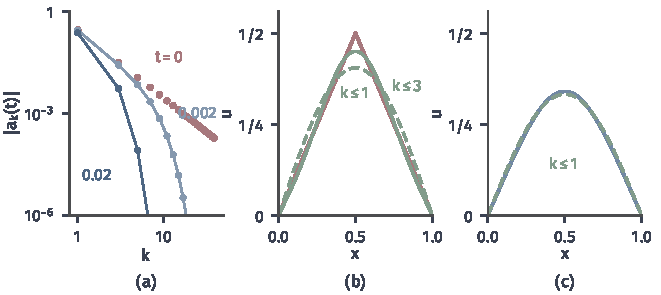
\includegraphics[width=112mm]{figures/06-differential-equations/02-partial-differential-equations/matplotlib/heat-tent-series/figure.pdf}
  \caption{三角形初值的正弦展开。(a)奇数$k$上系数的绝对值$\lvert a_k(t)\rvert=\lvert c_k\rvert\mathrm{e}^{-\lambda_kt}$，红点$t=0$，蓝色点线$t=0.002,0.02$。(b)$t=0$：三角形（红）与$k\leq1$（绿色虚线）、$k\leq3$（绿色实线）的部分和。(c)$t=0.02$：真解（蓝）与$k\leq1$的部分和（绿色虚线）。}
  \label{fig:heat-tent-series}
\end{BookInlineFigure}

\paragraph{Neumann问题与平均值}
余弦基的情形把上面的论证逐字重复，只需注意$\lambda_0=0$。设$u_0\in L^2(0,1)$，$a_0=\int_0^1u_0\,\mathrm{d}x$，$a_k=\langle u_0,\tilde{e}_k\rangle$，解是
\begin{equation}
 u(x,t)=a_0+\sum_{k\geq1}a_k\mathrm{e}^{-k^2\pi^2t}\tilde{e}_k(x) .
 \label{eq:heat-cosine-solution}
\end{equation}
同样的Parseval计算给出
\[
 \lVert u(\cdot,t)-a_0\rVert_2\leq\mathrm{e}^{-\pi^2t}\lVert u_0-a_0\rVert_2 ,
\]
所以温度趋于初值的平均值。

对三角形，$a_0=1/4$。分部积分一次，$\int_0^1u_0\cos(k\pi x)\,\mathrm{d}x$等于$\bigl(2\cos(k\pi/2)-1-(-1)^k\bigr)/(k^2\pi^2)$。只有$k\equiv2\pmod4$时它不为零，等于$-4/(k^2\pi^2)$，于是
\[
 u(x,t)=\frac14-\sum_{k\equiv2\ (\mathrm{mod}\ 4)}\frac{8}{k^2\pi^2}\,\mathrm{e}^{-k^2\pi^2t}\cos(k\pi x) .
\]
最慢的非常数项是$k=2$，衰减率$4\pi^2$，比一般的上界$\pi^2$快。原因仍是对称：$\cos\pi x$关于中点反对称，三角形不含这一分量。例如$t=0.1$时，$\tfrac{2}{\pi^2}\mathrm{e}^{-0.4\pi^2}\approx0.0039$，所以中点温度约$0.2539$，端点温度约$0.2461$，与图~\ref{fig:heat-zero-mode}(a)一致。

\begin{BookInlineFigure}
  \centering
  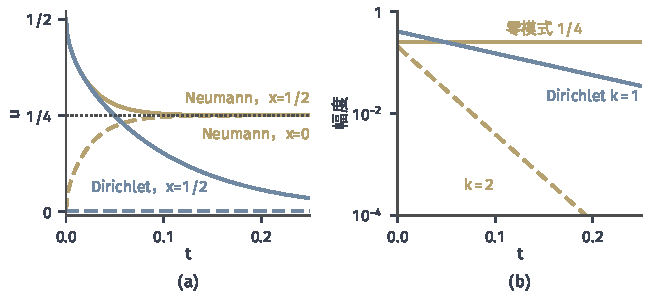
\includegraphics[width=112mm]{figures/06-differential-equations/02-partial-differential-equations/matplotlib/heat-zero-mode/figure.pdf}
  \caption{三角形初值下零模式的作用。(a)中点（实线）与端点（虚线）的温度：Neumann（黄）两条线都趋于$1/4$，Dirichlet（蓝）趋于$0$，蓝色虚线是固定为零的端点。(b)模式幅度，纵轴为对数：Neumann的常数模式$1/4$（黄实线）不变，$k=2$模式幅度$2\pi^{-2}\mathrm{e}^{-4\pi^2t}$（黄虚线）；Dirichlet最低模式幅度$4\pi^{-2}\mathrm{e}^{-\pi^2t}$（蓝）。}
  \label{fig:heat-zero-mode}
\end{BookInlineFigure}

\paragraph{不相容的初值}
定理~\ref{thm:heat-series}第一条的“$L^2$意义下”不是多余的谨慎。取$u_0=1$，两端仍固定为零，初值和边值在角点矛盾。系数是$c_k=\sqrt2(1-(-1)^k)/(k\pi)$，奇数项上为$2\sqrt2/(k\pi)$，于是$\sum_k\lvert c_k\rvert=\infty$，定理的第三条不能用。

$t=0$时部分和在$L^2$中收敛到$1$，但每个部分和在端点都等于$0$，而且靠近端点有固定幅度的过冲，这是\term{Gibbs现象}（Gibbs phenomenon）：奇延拓在端点有高度为$2$的跳跃，部分和的最大值趋于约$1.179$，取$k\leq61$时算得的最大值就是这个数，如图~\ref{fig:heat-corner-layer}(a)。

$t>0$时情形完全改变。定理第二条保证解光滑并且在端点为零，温度在边界附近形成一层过渡，图~\ref{fig:heat-corner-layer}(b)。层的厚度由$\sqrt{t}$决定：把横轴换成$x/(2\sqrt{t})$，不同时刻的层重合到同一条曲线，图~\ref{fig:heat-corner-layer}(c)，这条曲线的公式在下一节得到。

\begin{BookInlineFigure}
  \centering
  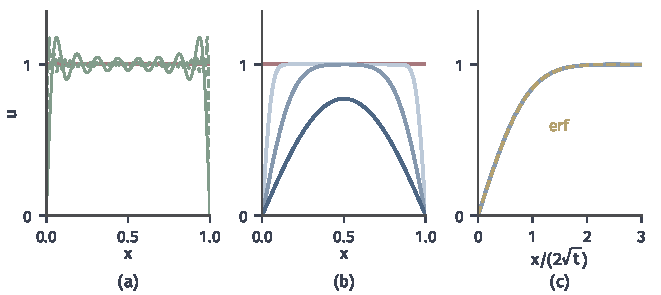
\includegraphics[width=112mm]{figures/06-differential-equations/02-partial-differential-equations/matplotlib/heat-corner-layer/figure.pdf}
  \caption{初值$u_0=1$与零边值不相容。(a)$t=0$：$k\leq15$（绿实线）与$k\leq61$（绿虚线）的部分和在红线附近振荡，端点旁有不随项数消失的过冲。(b)$t=0.001,0.01,0.05$的解（蓝色由浅到深），没有振荡。(c)$t=0.001$、$0.01$的边界层换成变量$x/(2\sqrt{t})$后重合，黄色虚线是$\operatorname{erf}$。}
  \label{fig:heat-corner-layer}
\end{BookInlineFigure}

于是，初值在什么意义下恢复取决于数据：一般的$L^2$初值在$L^2$意义下恢复；连续、分段可微且与边界相容的初值一致地恢复；与边界矛盾的初值在角点附近不可能一致地恢复，但这不妨碍$t>0$时的解是光滑的。
